\documentclass[12pt]{article}

%% Language and font encodings
\usepackage[english]{babel}
\usepackage[utf8x]{inputenc}
\usepackage[T1]{fontenc}
\usepackage{wrapfig}

%% Sets page size and margins
\usepackage[letterpaper,top=1in,bottom=1in,left=1in,right=1in,marginparwidth=1in]{geometry}

%% Useful packages
\usepackage{amsmath}
\usepackage{amssymb}
\usepackage{graphicx}
\usepackage[colorinlistoftodos]{todonotes}
\usepackage[colorlinks=true, allcolors=blue]{hyperref}

\newcommand{\Contributors}[1]{ {\footnotesize [\textit{#1}]}}

%A few journal ref commands
\newcommand{\apjl}{Astrophys. J. Lett.}
\newcommand{\apj}{Astrophys. J.}
\newcommand{\aap}{Astron. Astrophys.}
\newcommand{\nat}{Nature (London)}
\newcommand{\aj}{Astron. J.}
\newcommand{\prd}{Phys. Rev. D}
\newcommand{\aas}{Bull. Am. Astron. Soc.}
\newcommand{\mnras}{Mon. Not. R. Astron. Soc.}
\newcommand{\jcap}{Journal of Cosmology and Astroparticle Physics}
\newcommand{\vg}[1] {\textcolor{red}{#1}}

\title{\textbf{Astro2020 Science White Paper}\\
\vspace{0.5cm}
Cosmological Probes of Dark Matter: The Next Decade}
\date{}
\author{}

\begin{document}
\maketitle

\begin{abstract}
Cosmological observations offer unique and robust avenues for probing fundamental nature of dark matter particles---they broadly test a range of compelling theoretical scenarios, often surpassing or complementing the reach of terrestrial and other experiments.
We discuss observational and theoretical advancements that will play a pivotal role in realizing a strong program of cosmological searches for the identity of dark matter in the coming decade, with a focus on: CMB anisotropy and spectral distortions, and tracers of large-scale structure (Lyman-$\alpha$ forest, galaxy clustering and weak lensing, 21-cm tomography and sky-averaged signal).
This white paper is directed primarily to the ``Cosmology and Fundamental Physics'' panel of the Astro2020 Decadal Survey.  

\end{abstract}

\pagebreak
\section{Key Question: What is Dark Matter?}
 
Observations of the Universe, from our galactic neighbourhood, to the cosmological horizon, consistently testify that $\sim$85$\%$ of matter behaves as cold non-collisional fluid that sources gravitational potentials and underpins structure on virtually all observable scales.
\textbf{Over the past decades, it was confidently established that the main constituents of the dark matter (DM) component \textit{cannot} be any known baryonic particles.}
The existence of DM thus implies new physics whose investigation centrally drives research at the intersection of modern astrophysics and particle physics. 

Following its discovery, a versatile range of laboratory experiments was built worldwide to directly detect and/or produce some of the best-motivated particle candidates that could account for cosmological DM: WIMPs, WIMP-like particles, axions, etc; so far, this effort is without success.
Astrophysical and cosmological observations provide the only evidence for the existence of DM, and source a large portion of what is known about its properties---its stability on cosmological time scales, its apparent non-collisional nature, and its central role in the formation and growth of structure.
Recently, those observations have also emerged as a powerful probe of DM microphysics, complementary in reach to laboratory experiments.

%%%%%%%%%%%%%%%%%
\begin{wrapfigure}{r}{0.5\textwidth}
\begin{center}
\vspace{-0.9cm}
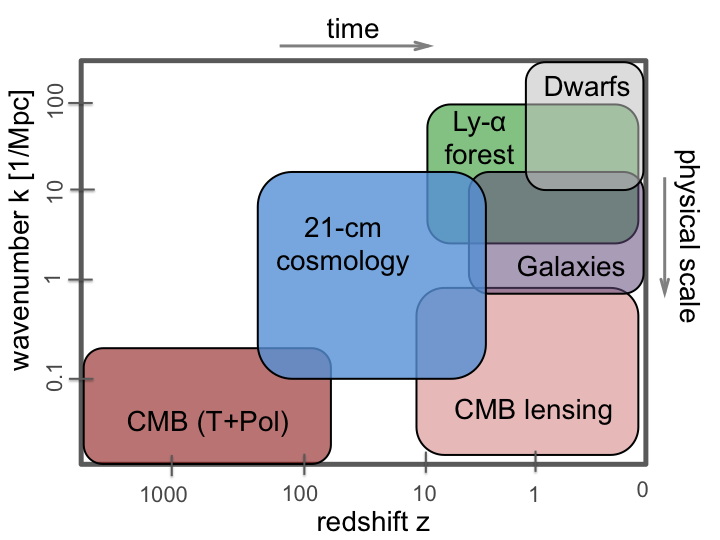
\includegraphics[width=0.5\textwidth]{scales.png}
\end{center}
\vspace{-0.8cm}
\caption{Approximate mapping of different observables onto cosmological epochs and physical scales (spectral distortions are omitted for compactness of presentation; their range is outside the LHS border of the plot).}
\vspace{-0.1cm}
\label{fig:scales}
\end{wrapfigure}
%%%%%%%%%%%%%%%%% 
We focus on cosmological searches for DM particles, whose key goal is to detect the effects of DM interactions on density fluctuations and thermal history of the Universe, and use them to pin down particle identity of DM.
\textbf{Cosmology is a versatile tool that can uniquely address broad classes of well-motivated theoretical scenarios}: DM interactions with known particles (baryons, photons, and neutrinos), interactions within the DM sector itself, and DM annihilations and decays.\footnote{We note that other science white papers focus on alternative scenarios in which DM consists of ultra-light axion-like particles, warm DM, primordial black holes, etc.}
In this physical context, we review strengths, caveats, and future promise of a range of cosmological probes.
{Different observables test the same underlying microphysics in mutually complementary ways---by probing its signatures throughout cosmic history, on a broad range of physical scales} (illustrated in Fig.~\ref{fig:scales}).
\textbf{Establishing a discovery of DM signals and robust tests of its fundamental nature require independent confirmation and consistency checks between all available observations.}
Central to this will be the effort to understand synergies between observables and enable their joint analyses in the coming decade.
We will conclude with a list of advancements that will play a pivotal role in this program.
%%%%%%%%%%%%%%%%%%%%%%%%%%%%%%%%%%%%%%%%%%%%%
\section{Theory and Observations}
\label{sec:thobs}
%\vspace{-0.2cm}}
\subsection{Scattering with Baryons}

In the standard model of cosmology DM is non-collisional, but elastic scattering between DM and visible particles is commonplace in some of the best-motivated DM models, including the WIMPs and WIMP-like particles.
For this reason, the most sensitive terrestrial DM searches with direct detection experiments are looking for scattering of Galactic-halo DM on nuclei in underground targets.
However, the same scattering processes can occur in a cosmological setting and lead to an exchange of heat and momentum between DM and baryons, absent in the standard (non-collisional) cosmology. 
This can affect both the thermal history of the Universe and the evolution of cosmological perturbations, captured by various observables.

%%%%%%%%%%%%%%%%%%%%%
\textbf{CMB spectral distortions.} 
DM can drain heat from the primordial plasma, by scattering with either protons, electrons, or photons, in the early Universe \cite{AliHaimoud_15}.
Energy exchange between DM and the photon-baryon fluid occurring later than two months after the Big Bang cannot fully thermalize, and thus leads to distortions of the CMB frequency spectrum away from a perfect blackbody \cite{Hu_96,Chluba_13}.  
%The rate of heat transfer is proportional to the \emph{number density} of DM particles, and hence inversely proportional to their mass. 
The CMB frequency spectrum is most sensitive to light particles that thermally decouple as early as $z \sim 2 \times 10^6$.
The existing COBE FIRAS measurements provide upper limits on DM-baryon and DM-photon interactions, for DM masses lower than $\sim 0.1$ MeV. 
These limits are similarly stringent, but independent of those derived from CMB anisotropy from \textit{Planck}.
Future measurements that can detect a fractional distortion of order $\sim 10^{-8}$ would be sensitive to interacting DM particles as massive as $\sim 1$ GeV. 
Spectral distortions in conjunction with power-suppression in CMB anisotropy in future data could yield robust evidence for DM physics taking place in the early Universe.

%%%%%%%%%%%%%%%%%%%%%%%%%%%%%%%%%%%%
\textbf{CMB anisotropy.} 
Scattering in the early Universe (prior to recombination at $z\sim 1100$) leads to momentum transfer and a drag force between the DM and the baryon fluids.
This results is power suppression in density fluctuations that is more prominent on progressively smaller scales, with an amplitude inversely proportional to the strength of the scattering interaction.
As perturbations grow, the lack of small-scale structure propagates into all visible tracers of matter, and shows up in observables that span cosmic history (Fig.~\ref{fig:scales}).
%%%

\textit{Planck} measurements of the CMB temperature anisotropy currently provide the most pristine cosmological bound on DM-baryon scattering cross section~\cite{Boddy:2018kfv,Gluscevic:2017ywp,Boddy:2018wzy,Xu:2018efh,Slatyer:2018aqg,Dvorkin:2013cea}; they already sensitively probe DM interactions as far back in time as when the Universe was a thousand years old.
However, the first high-signal-to-noise measurements of the CMB polarization and lensing anisotropy on small angular scales---to be delivered by the next-generation ground-based CMB experiments---can enable a leap in sensitivity to DM scattering by \textit{orders of magnitude}~\cite{Li:2018zdm}.
Interestingly, the effects of DM-baryon interactions are distinct from other new physics targeted by ground-based CMB experiments (such as, for example, the neutrino mass and ultra-light particles).
Furthermore, DM-baryon scattering is not sensitive to the uncertainties on cosmological parameters, and can thus be robustly probed with the CMB.
However, in spite of its robustness, CMB has a limited grasp of small scales where the effects of interactions are more prominent; small scales are accessible to other observables, but are more prone to modeling and measurement systematic uncertainties.

\textbf{Lyman-$\alpha$ forest.} 
For example, the Lyman-$\alpha$ forest measurements from \vg{SDSS-2} trace matter power spectrum on scales of about 1 Mpc comoving; their analysis has provide the most stringent to-date cosmological bound on DM-baryon interactions, surpassing the reach of the CMB  \cite{Dvorkin:2013cga,Slatyer:2018aqg,Xu:2018efh}.
This bound implies that a baryon withing a galaxy like the Milky Way does \textit{not} scatter with DM over the age of the galaxy.
There is vast room for improvement with future spectroscopic surveys that could reconstruct even smaller scales with similar measurements.
However, inference of fundamental physics from these measurements will crucially rely on accurate modeling of the Lyman-$\alpha$ forest and non-linear evolution of small scales.
Consistency checks and joint analyses with high-precision CMB measurements and other probes may help alleviate such uncertainties in future data.

%%%%%%%%%%%%%%%%%%%%%%%%%%
\textbf{21-cm cosmology.} 
Over the coming decade, measurements of the hyperfine 21-cm line transition in atomic hydrogen gas during cosmic Dark Ages and cosmic reionization ($10<z<1000$) may start to probe redshifts far beyond the reach of current observations.
The strength of the 21-cm signal is proportional to the difference between the temperature of the hydrogen gas (baryons) and that of the CMB, and can serve as a calorimeter that probes thermal history at redshifts as high as $\sim 200$ \cite{Loeb_04, Breysse_18}.
If DM-baryon scattering occurs \textit{after} recombination is complete, it can alter thermal evolution of baryons in the epoch originating the 21-cm signal. 
The sky-averaged signal and its fluctuations are both sensitive to this effect \cite{Munoz_15, Barkana_18, Fialkov_18, Munoz_18}.
Such late-time scattering scenario, for example, arises if DM particles carry a small electric charge and exhibit Coulomb-like interactions (``millicharged'' DM).
This scenario is simple and well-motivated, but challenging to probe in direct detection experiments and is an excellent example of a model where cosmological probes may present an optimal detection channel.
However, cosmological 21-cm signal is exceptionally hard to detect due to the size of galactic foreground emission at the same frequencies. 
As was recently demonstrated on the example of the EDGES anomaly \cite{}, a combination and consistency checks with other probes may be essential for interpretation of future signals as new physics. 

%%%%%%%%%%%%%%%%
\textbf{Galaxies.}
Galaxies (and their satellites) trace matter power spectrum on even smaller scales (and in the local Universe), and thus hold a bold promise as a future probe of DM physics \cite{2019arXiv190201055D}.
Given the physical scales involved, studies of dwarfs in particular, could unlock orders of magnitude improvement in sensitivity to DM interactions, over high-redshift and large-scale probes discussed until this point.
However, robust inference of fundamental physics from studies of galaxies will crucially depend on improvements in modeling and numerical simulation of their formation, non-linear growth, and baryonic effects in cosmologies with non-standard DM---a challenge that will need much attention in the coming decade.\footnote{Observables such as galaxy clustering and weak lensing are a large subject and a prime focus of other science white papers.}

%%%%%%%%%%%%%%%%%%%%%%%%%%%%%%%%%%%%%%%%%%%%%%%
\vspace{-0.3cm}
\subsection{Scattering with Neutrinos}

Neutrinos reside in the part of the Standard Model of particles that is the least well understood; indeed non-vanishing neutrino masses already require new physics to explain. 
In addition, terrestrial neutrino experiments and probes of astrophysical neutrinos have recently seen a number of intriguing anomalies that may signify new physics \cite{miniboone, others, ANITA}, making the idea of a DM-neutrino interaction of interest from several perspectives. 
However, laboratory neutrino experiments remain extremely challenging, and exploration of DM-neutrino interactions in such setting is currently impossible. 
On the other hand, neutrinos are cosmologically important owing to their high abundance (on the order of 100 per cm$^3$ today).
If neutrinos interact efficiently with DM particles at the time the standard neutrino decoupling takes place (when the temperature of the Universe is about 1 MeV), tightly-coupled DM-neutrino fluid undergoes acoustic oscillations and diffusion damping. 
The net effect is suppression of small-scale power in matter fluctuations, similar to that in the case of DM-baryon scattering \cite{Boehm:2001hm,Mangano:2006mp}.
Gravitational interactions between neutrinos and photons are sensitively captured by CMB anisotropy measurements.
In presence of DM-neutrino scattering, photons interact with a DM-neutrino fluid, which is smoother than ordinary free-streaming neutrinos, and has a smaller sound speed. 
This tends to suppress the CMB acoustic peaks and to shift them to smaller angular scales \cite{Wilkinson:2014ksa}. 
Bounds on DM-neutrino interactions were already placed using CMB anisotropy measurements from \textit{Planck}  \cite{Escudero:2015yka,DiValentino:2017oaw,Diacoumis:2018ezi}.
However, just like the case of scattering with baryons, the effects of DM-neutrino interactions are more prominent on smaller scales, and so the current bounds are by far dominated by Lyman-$\alpha$ forest observations \cite{Wilkinson:2014ksa}.
However, in the case of a positive detection of a suppression in the matter power spectrum reconstructed with future Lyman--$\alpha$ data, high-precision CMB data could serve as a cross check and offer an opportunity to discriminate between various candidate models.

%%%%%%%%%%%%%%%%%%%%%%%%%%%%%%%%%%%%%%%%%%
\vspace{-0.3cm}
\subsection{Annihilation and Decay}

If DM interacts with visible particles, it may also annihilate or decay and that way further alter the thermal history of the Universe. 
If annihilation or decay products include electromagnetically interacting particles, these particles and their decay products can generically heat and/or ionize the baryonic gas.
Cosmological searches have distinct advantages over classic indirect searches for DM annihilation and decay, as they do not suffer from astrophysical backgrounds and large uncertainties in the distribution of DM in the target systems.
Furthermore, they can probe processes which have no detectable signals in terrestrial-scale experiments and in the local Universe--for example, the decay of metastable species with lifetimes comparable to the age of the Universe, and decay of DM particles into invisible channels, such as neutrinos or new dark particles \cite{Poulin:2016nat,Poulin:2016anj}. 

Increasing the ionization fraction near the time of recombination can affect the CMB anisotropy \cite{Adams:1998nr,Chen:2003gz, Padmanabhan:2005es,Dvorkin:2013cga}. 
\textit{Planck} measurements of CMB temperature on large angular scales provided some of the strongest and most robust bounds on annihilations and decays of sub-GeV DM, complementing indirect searches that probe heavier DM candidates \cite{Aghanim:2018eyx,Slatyer:2016qyl}. 
Measurements from the next-generation ground-based CMB experiments can improve sensitivity to DM annihilation cross section and lifetime by a factor of several.
%In addition, heating of the photon-baryon plasma by DM annihilation and decay in pre-recombination Universe, and production of secondary low-energy photons, could  distort the frequency spectrum of the CMB; however, the expected fractional distortion is exceedingly small ($\sim 10^{-9}-10^{-10}$) \cite{Chluba:2013wsa,Chluba:2016bvg}.
Furthermore, as discussed in context of DM-baryon interactions, future observations of the cosmological 21-cm signal from atomic hydrogen can sensitively track gas temperature during cosmic Dark Ages and around the epoch or Reionization.
As such, they can capture any new energy injection from DM decays and annihilations in post-recombination Universe, likely surpassing the sensitivity of the CMB anisotropy to the same processes \cite{Furlanetto:2006wp,Valdes:2007cu,Evoli:2014pva,Lopez-Honorez:2016sur,Poulin:2016anj}. 

%%%%%%%%%%%%%%%%%%%%%%%%%%%%%%%%%%%%%%%%%%%%%%%%
\vspace{-0.3cm}
\subsection{Interactions with Dark Radiation}

Models in which the dark sector is complex and contains not only dark matter, but also dark radiation (DR) that interacts with DM particles, are motivated in several ways: they generically arise in theories proposed to explain the hierarchy problem of the Standard Model of particles \cite{Arkani-Hamed:2016rle, Chacko:2018vss}; they could explain the anomalously low large-scale amplitude of matter fluctuations seen in some weak-lensing surveys \cite{Lesgourgues:2015wza,Chacko:2016kgg,Buen-Abad:2017gxg,Krall:2017xcw}; they present a specific case of self-interacting DM, an attractive potential solution for putative anomalies on sub-galactic scales, such as the missing-satellite problem \cite{Tulin:2012wi,Tulin:2013teo,Kaplinghat:2015aga,Bullock:2017xww}. 
Cosmology offers a unique venue for probing yet-unknown DM--DR interactions, especially if DM resides in a secluded dark sector featuring only weak coupling to known particles.

Similar to how photon pressure prohibits growth of baryon fluctuations until the epoch of recombination, the DM fluid interacting with DR in the early Universe experiences suppressed growth of structure, as compared to a scenario with no DR. 
The power suppression is reflected in the CMB anisotropy and in all tracers of large-scale structure, similar to the case of DM-baryon interactions: galaxy clustering, weak gravitational lensing, Lyman-$\alpha$ forest, and 21-cm tomography \cite{Boehm:2001hm,Cyr-Racine:2013fsa,Cyr-Racine:2015ihg}. 
Notably, cosmological signatures of DR are distinct from signatures of relativistic particles that do not couple to DM, such as the standard free-streaming neutrinos~\cite{Bashinsky:2003tk,Follin:2015hya,Baumann:2015rya}.
In the coming decade, high-precision measurements of small-angular-scale CMB polarization anisotropy with the next-generation ground-based experiments could robustly detect or rule out DM-DR interactions taking place at redshifts below $\sim10^6$, even in the case where only a small fraction (less than $5\%$) of the overall DM density experiences interactions with DR. 
As in the other theoretical scenarios, Lyman-$\alpha$ forest and 21-cm observations could extend the sensitivity to DM--DR interactions taking place at even smaller scales and earlier times. 

\vspace{-0.3cm}
\section{Recommendations}
\label{sec:recommendations}
\vspace{-0.2cm}
Cosmological observations offer unique and robust avenues for probing physical nature of dark matter particles---they broadly test a range of compelling theoretical scenarios, often surpassing or complementing the reach of terrestrial experiments.
The following advancements will play a pivotal role in realizing a strong program of cosmological searches for the identity of dark matter in the coming decade:
\begin{itemize}
    \item \textbf{Observations:}
    \begin{itemize}
        \item Ground-based measurements of small-angular-scale CMB anisotropy.
        \item Surveys of matter-power-spectrum tracers (21-cm tomography, Lyman-$\alpha$ forest, galaxy clustering and weak lensing).
        \item Observations of thermal-history tracers (sky-averaged 21-cm signal, CMB spectral distortions).
        \item Near-field cosmology (studies of statistical properties of dwarf galaxies).
    \end{itemize}
    \item \textbf{Theory and analysis:}
    \begin{itemize}
        \item Simulation and modeling of non-linear growth in novel DM cosmologies.
        \item Understanding of baryonic systematic effects in inferrences about DM physics.
        \item Frameworks for joint analyses of cosmological probes.
        \item High-accuracy theoretical tratment of cosmological DM signals. \end{itemize}
\end{itemize}
\bibliographystyle{ieeetr}
\bibliography{DMCosmology}

\end{document}